%%%%%%%%%%%%%%%%%%%%%%%%%%%%%%%%%%%%%%%%%%%%%%%%%%%%%%%%%%%%%%%%%%%%%%%%
% Preamble
%%%%%%%%%%%%%%%%%%%%%%%%%%%%%%%%%%%%%%%%%%%%%%%%%%%%%%%%%%%%%%%%%%%%%%%%
\documentclass[11pt]{article}
%
% Packages and other includes
% Pagination
\usepackage[letterpaper, margin=1.25in]{geometry}
%
% Graphics, floats, tables
\usepackage{graphicx, xcolor, float, array}
%
% Fonts
\usepackage[T1]{fontenc} % best for Western European languages
\usepackage{lmodern} % Latin Modern instead of CM
\usepackage{textcomp} % required to get special symbols
%
% Math
\usepackage{amsmath, amssymb}
\usepackage{enumerate}
\usepackage{braket}
\usepackage{wrapfig}
% 
% Hyperlinks
\usepackage[colorlinks,linkcolor={red},citecolor={blue},
urlcolor={blue}]{hyperref} 
%
% Definitions and settings
% Paragraph indent and spacing
\setlength{\parskip}{0.4\baselineskip}
\setlength{\parindent}{0in}

\renewcommand{\theenumi}{\alph{enumi}}
\renewcommand{\labelenumi}{\theenumi)}
\renewcommand{\theenumii}{\roman{enumii}}

\newcommand{\filipp}[1]{{\color{purple} #1 }}


\newcounter{problem}
\newcommand{\problem}[2]{\stepcounter{problem}\textbf{{\theproblem}.\,
    {#1}} (#2 credits)}

\newcommand{\answer}[2]{
  \framebox{\begin{minipage}{\linewidth}
      Answer {#2}: \vspace*{#1}
  \end{minipage}
  }
}

\begin{document}

\hfill 03/14/2022
\begin{center}
\textbf{\large Honors General Chemistry (Chem H2B) Winter
  2022 \\ Final Exam}
\end{center}

\subsection*{Instructions}

\begin{itemize}
\item Answer the questions below in the spaces provided. For full
  credit, results must be \emph{inside} the answer boxes, rounded exactly
  to the requested precision, and in the correct units. 
\item If you need additional space for your work, use separate sheets of
  paper (provided to you during the exam), and submit them together with
  the exam. Do not write on the back of any sheet.
\item This exam is administered in person and closed book. You may use a
  calculator and a hand-written 4"$\times$6" note card (with writing on
  both sides), but no other electronic devices, notes, or books are
  allowed. 
\item This exam comprises 11 problems on 7 pages (excluding the cover page).
\item Constants, unit conversions, and useful identities are provided in
  the appendix. 
\item Please use only the molar masses provided in each
  problem and the exact values of the constants provided in the
  Appendix. Do not take atomic weights from the periodic table.
\item Do not round intermediate results.
\item Exam time is 120 minutes.
\end{itemize}

\vfill

\textbf{By submitting this exam, you certify under the penalty of an
  academic integrity violation that all results are your
  own and were obtained according to the rules above. You consent to
  be forthcoming to any subsequent questions about your results and how
  exactly they were obtained, and understand that you may not receive
  credit if you cannot give a satisfactory answer.}

\vfill

\subsection*{Problems}

\problem{Ammonia Fuel Cell}{4}

Ammonia fuel cells use oxygen from the air to combust ammonia gas. In
modern cells, the exhaust contains only dinitrogen and water.

\begin{enumerate}
  \item Formulate the balanced chemical equation for the combustion
    reaction, including states.
    
    \answer{0.2in}{}

  \item How many grams of ammonia are necessary to generate 1 kWh of
    electricity at standard conditions? Assume that the fuel cell
    operates at 99\% efficiency. The standard free enthalpies of
    formation of ammonia gas and liquid water are $-16.4$ kJ/mol and
    $-237.1$ kJ/mol, respectively.

    \vfill 

    \answer{0.2in}{(3 significant figures)}

  \end{enumerate}
    
    
\problem{Hess's Law}{4}

Ethyne (a.k.a. acetylene,  C$_2$H$_2$) is commonly used in
welding. Ethyne gas may be synthesized by reaction of 
calcium carbide (CaC$_2$) with water.

You are given the following data:
\begin{align*}
  \text{CaO(s) + H$_2$O(l)} & \rightarrow \text{Ca(OH)$_2$(s)}
  \hfill & \Delta H^\circ_r = -65.3\text{ kJ/mol} \\
  \text{2 CaO(s) + 5 C(s,graphite)} & \rightarrow \text{2 CaC$_2$(s) + CO$_2$(g)}
  \hfill & \Delta H^\circ_r = 753.1\text{ kJ/mol} \\
  \text{CaC$_2$(s) + 2 H$_2$O(l)} & \rightarrow \text{Ca(OH)$_2$(s) + C$_2$H$_2$(g)}
  \hfill & \Delta H^\circ_r = -126.2\text{ kJ/mol} \\
  \text{C(s,graphite) + O$_2$(g)} & \rightarrow \text{CO$_2$(g)}
  \hfill & \Delta H^\circ_r = -393.5\text{ kJ/mol} \\
  \text{2 H$_2$O(l)} & \rightarrow \text{2 H$_2$(g) + O$_2$(g)}
  \hfill & \Delta H^\circ_r = 571.8\text{ kJ/mol}
\end{align*}

\begin{enumerate}
\item Write the chemical equation for the formation of C$_2$H$_2$
  including states. 
  
  \answer{0.2in}{}
\item Determine the standard enthalpy of formation of gaseous ethyne.

  \vfill
  \answer{0.2in}{(3 significant figures)}
\end{enumerate}

\problem{Mixing Ideal Gass}{6}

At 25$^\circ$C, equal volumes pure nitrogen dioxide and
pure dinitrogen tetroxide are initially separated by a valve, see
Figure \ref{fig:mix}. The initial pressure of
both gases is 1.25 atm. The valve is then opened, allowing
the gases to mix. Assume ideal gas behavior in the following.

\begin{figure}[hbpt]
  \centering
  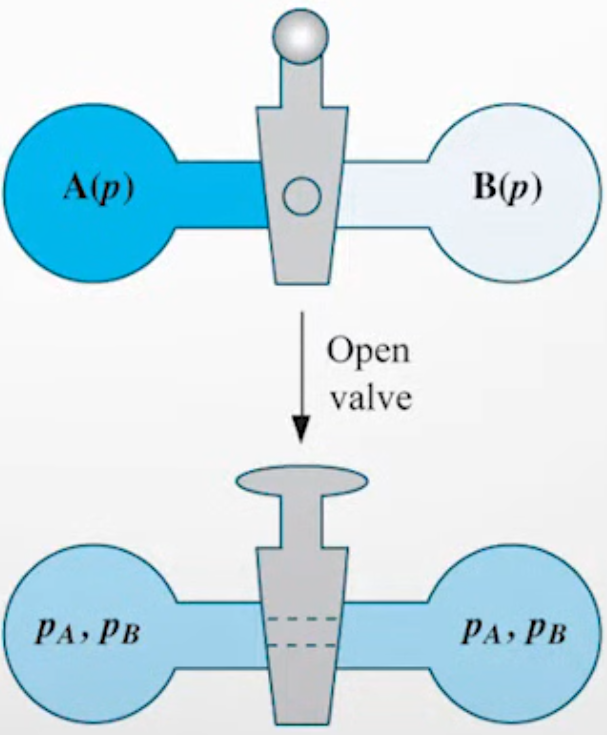
\includegraphics[scale=0.22]{mix_ideal.png}
  \caption{Two gases A and B separated into equal volumes.}
  \label{fig:mix}
\end{figure}

\begin{enumerate}
  
\item Dinitrogen tetraoxide is in equilibrium with nitrogen dioxide.
  Formulate the balanced chemical equation including states.

  \answer{0.2in}{}
\item Determine the free energy of mixing $\Delta G_\text{mix}$.

  \vfill
  
  \answer{0.2in}{(2 significant figures)}

\item At 25$^\circ$C, the equilibrium constant $K$ for dissociation of
  dinitrogen oxide is 0.1481. What are the thermodynamic driving forces
  making the gases (i) mix and (ii) equilibrate spontaneously?

  \answer{1in}{}
\end{enumerate}

\pagebreak

\problem{Gas Equilibrium}{5}

Phosgene (COCl$_2$) is a toxic, colorless gas used in the
manufacturing of polyurethanes and polycarbonate plastics. At
$527^\circ$C, it decomposes into carbon monoxide and chlorine. 

\begin{enumerate}
\item Formulate the balanced chemical equation for the decomposition of
  COCl$_2$, including states. 

  \answer{0.2in}{}
  
\item At $527^\circ$C, the equilibrium constant $K$ is $3.08\times 10^{-4}$.
  Given the thermodynamic data in Table \ref{tab:cocl2}, determine $K$ at
  50$^\circ$C. 

  \begin{table}[htbp]
  \begin{center}
    \begin{tabular}{ll}
      Compound & $\Delta$ H$_f^{\circ}$ (kJ/mol) \\
      \hline
      Phosgene        & $-220.92$  \\
      Carbon Monoxide & $-110.54$  \\
      Chlorine        & $0$
    \end{tabular}
  \end{center}
  \caption{Standard enthalpy of formation data.}
  \label{tab:cocl2}
  \end{table}

  \vfill
  
  \answer{0.2in}{(3 significant figures)}
  
\end{enumerate}

\problem{Essay Question: Intermolecular Interactions}{4}

The boiling points of methanol, methanethiol, and methaneselenol are
65$^{\circ}$C, 6$^{\circ}$C, and 12$^{\circ}$C. Explain in a few
sentences what types intermolecular interactions are present in each of
these cases, and give a rationale for the trend in the observed boiling
points. Why does methanethiol have the lowest boiling point of all three?

\answer{2.5in}{}

\problem{Boiling Points and Vapor Pressures}{4}

Consider the following compounds: water, decane, sulfuric acid, and
methanol. 

\begin{enumerate}
\item Order the above compounds by decreasing volatility.
  
  \answer{0.2in}{}

\item Order the above compounds by decreasing boiling point.
  
  \answer{0.2in}{}
\end{enumerate}

\problem{Colligative Property of Solutions}{4}

An aqueous solution contains $10.5\%$ NaCl by mass. What is the
substance amount of water in mol 
contained in 2.5 L of the vapor above the solution at 55$^\circ$C? The
vapor pressure of pure water at 55$^\circ$C is 118 torr. Assume ideal
behavior.  

\vfill

\answer{0.2in}{(3 significant figures)}

\pagebreak

\problem{Statistical Thermodynamics}{7}

Dairy farms accounted for approximately $10\%$ of greenhouse gas emissions in
2019, according to the US Environmental Protection Agency. Some farms
use manure to convert it to methane gas, which may be used, e.g., for
electricity generation. Assume ideal gas conditions in the following. 
\begin{figure}[hbpt]
  \centering
  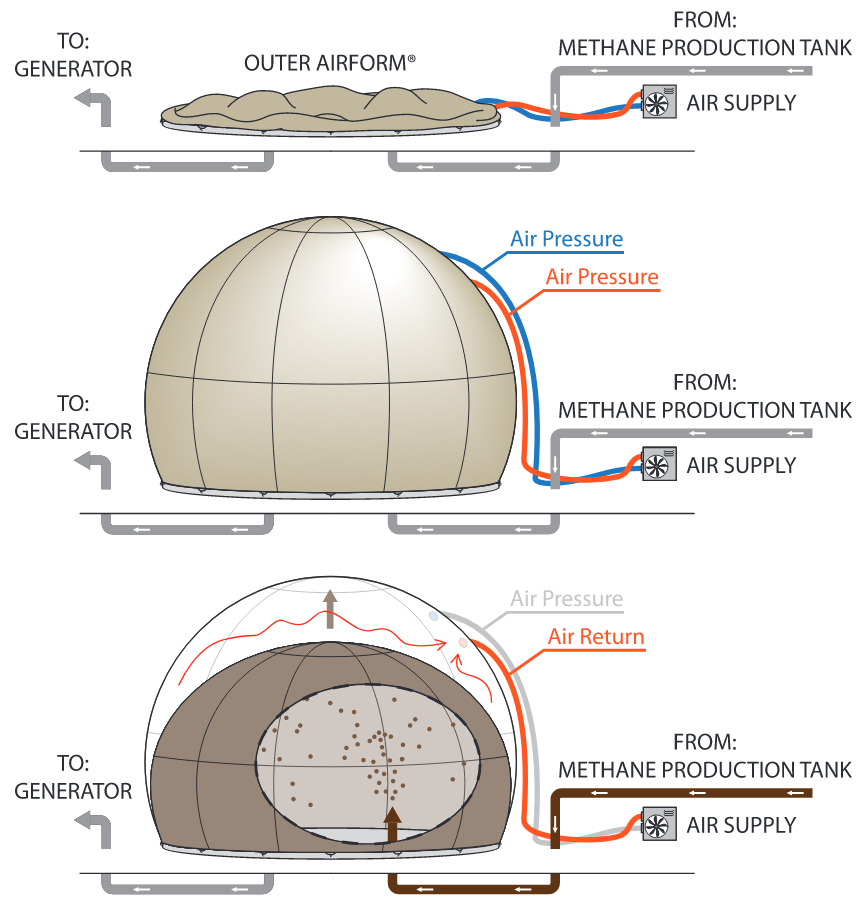
\includegraphics[scale=0.25]{tank_store.png}
  \label{fig:ch4}
\end{figure}
\vspace{-0.25in}
\begin{enumerate}
\item Methane gas is stored in an airtight tank, see Figure
  \ref{fig:ch4}. Determine the total enthalpy of 10 kg of methane
  stored at 300 K.

  \vfill
  
  \answer{0.2in}{(3 significant figures)}

\item Estimate the root mean square velocity of the methane molecules in m/s at
  300 K. The molecular mass of methane is $2.665\times 10^{-26}$ kg.

  \vfill
  
  \answer{0.2in}{(3 significant figures)}

\item On a warm day, the tank expands from 15 L to 17.5 L. Estimate the
  molar heat capacity $C_{p,m}$ in multiples of the ideal gas constant $R$
  using the equipartition theorem. 

  \vfill
  
  \answer{0.2in}{}

\item Compute the change in internal energy for this state change.

  \vfill
  
  \answer{0.2in}{(3 significant figures)}

\end{enumerate}


\problem{Boiling Water at High Elevation}{8}

The barometric formula is 
\begin{equation*}
  P_h = P_0 e^{-\frac{Mgh}{RT}}
\end{equation*}
where $P_h$ is the pressure at height $h$, $P_0$ is the pressure at
sea level, $M$ is the molar mass of air (28.97 g/mol), $R$ is the ideal
gas constant, and $T$ is the temperature. Report to 3 significant figures.

\begin{enumerate}
\item Before hiking to the peak of Mt. Everest, hikers often make a stop
  at the Everest base 
  camp in Nepal. The altitude is 5,364 m. Approximate the atmospheric
  pressure at the base camp given that the pressure at ground level and
  25$^\circ$C is 760. torr. 

  \vfill
  
  \answer{0.2in}{(3 significant figures)}

\item At the Everest base camp, what temperature does the water boils at?
  Assume the enthalpy of vaporization of water $\Delta H_\text{vap}$ is 40.7 kJ/mol.

%  Estimate the new temperature at which water boils at. \filipp{not sure what you
%    want here}

  \vfill
  
  \answer{0.2in}{(3 significant figures)}

\item Use the value in part b), how much energy is needed to convert 1 L of ice
  (density is 0.917 g/mL) at -10$^\circ$ into steam? Assume the specific
  heats of ice and water are 2.093 J/(g $^\circ$C) and 4.186 J/(g $^\circ$C),
  respectively. The $\Delta H_\text{fus}$ is 6.01 kJ/mol.
%  \filipp{what do you mean by ``completely
%    boil''?}

  \vfill
  
  \answer{0.2in}{(3 significant figures)}
\end{enumerate}

\pagebreak

\problem{Essay Question: Properties of Water}{4}

\begin{enumerate}
\item Water has unique properties that allow life to thrive on Earth. Explain in
  a few sentences how water plays a key role in regulating the Earth's climate.
  Include in your asnwer at least one relevant property of water.

  \answer{1in}{}

\item Based on the phase diagram in Figure \ref{fig:h2o}, why is the solid-liquid
  slope steep and negative? \textit{Hint:} Gibbs--Duhem 
  equation $\sum_i N_i\Delta\mu_i = V\Delta P - S\Delta T$
%  \filipp{make a separate problem.}

  \begin{figure}[hbpt]
    \centering
    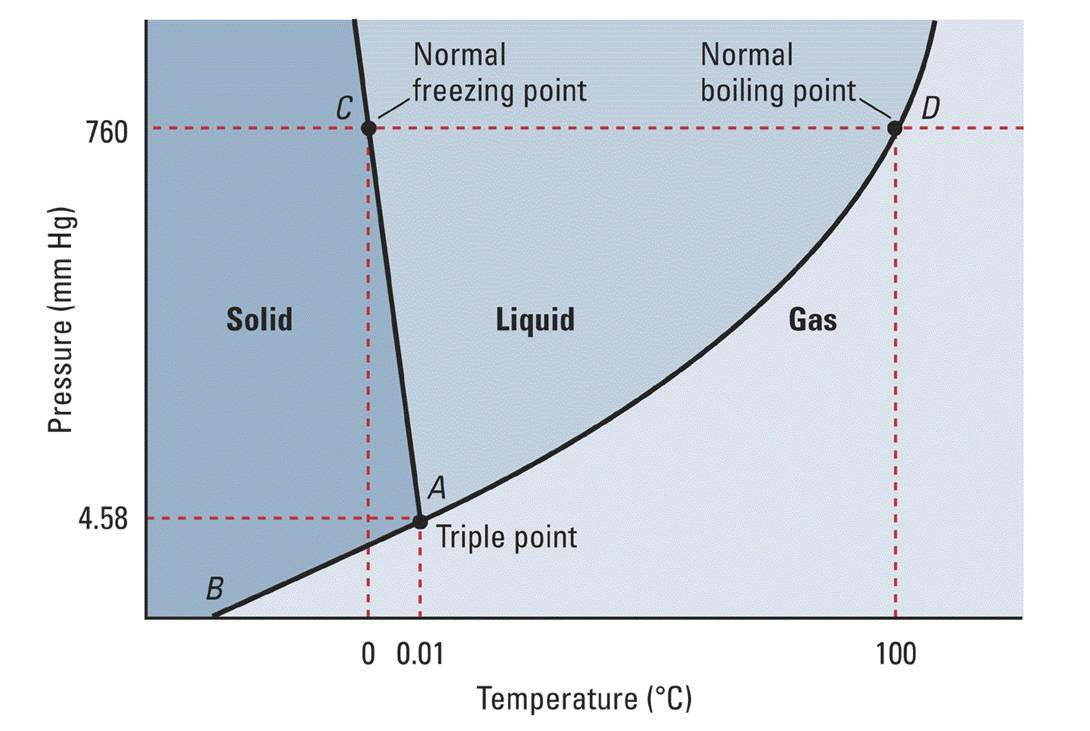
\includegraphics[scale=0.2]{water_phase.jpg}
    \caption{Phase diagram of water}
    \label{fig:h2o}
  \end{figure}

  \answer{1in}{}
\end{enumerate}

\problem{Extra Credit: Crystal Structures}{3}

Classify the following solids as molecular, covalent, ionic, and metallic solids:
polonium, ammonium sulfate, silicon dioxide (sand), ice, and graphite.

\answer{0.5in}{}

%\filipp{This one is tough. I think they may perceive asking this question as
%  unfair, even if it is extra credit... Perhaps replace by asking
%  them to categorize a few solids as metals, ionic, network, or molecular.}
%
%Potassium exists as a body-centered cubic (bcc) crystal and the lattice constant is $5.328 \AA$.
%
%\begin{enumerate}
%\item How many potassium atoms are in a single bcc unit cell?
%
%  \answer{0.2in}{}
%  
%\item Determine the atomic radius of potassium.
%
%  \answer{0.2in}{}
%  
%\item Calculate the density of potassium.
%  
%  
%\end{enumerate}

\vfill

\clearpage

\subsection*{Appendix A: Constants and Unit Conversions}

\begin{table}[htbp]
  \begin{tabular}{lll}
    Constant & Symbol & Value \\
    \hline
    Ideal gas constant & $R$ & 8.3145 J/(mol K) \\
    Boltzmann constant & $k$ & 1.3806$\times 10^{-23}$ J/K \\
    Avogadro's constant & $N_A$ & 6.022 $\times 10^{23}$ mol$^{-1}$ \\
    Standard temperature (STP) & $T_s$ & 273.15 K \\
    Standard pressure (STP) & $P_s$ & 101325 Pa = 1 atm \\
    Molar volume of an ideal gas at STP & $v_s$ & 22.414 L/mol \\
    Standard thermodynamic pressure & $P^{\circ}$ & 100 kPa \\
  \end{tabular}
  \caption{Physical constants}
  \label{tab:const}
\end{table}

\bigskip

\begin{table}[htbp]
  \begin{tabular}{ll}
    Quantity & Conversion \\
    \hline
    Volume & 1 gal = 3.7854 L \\
    Temperature & $\theta_C/{^\circ} C = \left (\theta_F/F - 32
    \right ) \times \frac{5}{9}$ \\
    Pressure & 1 atm = 101325 Pa = 760 torr \\
    Energy & 1 kWh = $3.6\times 10^6$ J
  \end{tabular}
  \caption{Unit conversions}
  \label{tab:const}
\end{table}


\subsection*{Appendix B: Identities}

Free energy change of an isothermal gas expansion:

\begin{equation*}
  G(P) = G^\circ + nRT\ln\frac{P}{P^\circ}
\end{equation*}

Van't Hoff Equation:
\begin{equation*}
  \ln K = -\frac{\Delta H^\circ}{RT} + \frac{\Delta S^\circ}{R}
\end{equation*}

Average kinetic energy:
\begin{equation*}
  E_{\text{kin}} = \frac{1}{2} m v_{\text{rms}}^2
\end{equation*}

Clausius--Clapeyron Equation:
\begin{equation*}
  P_f = P_ie^{-\frac{\Delta H_\text{vap}}{R}(\frac{1}{T_f} - \frac{1}{T_i})}
\end{equation*}

\clearpage

\subsection*{Appendix C: Periodic Table of the Elements}

\begin{center}
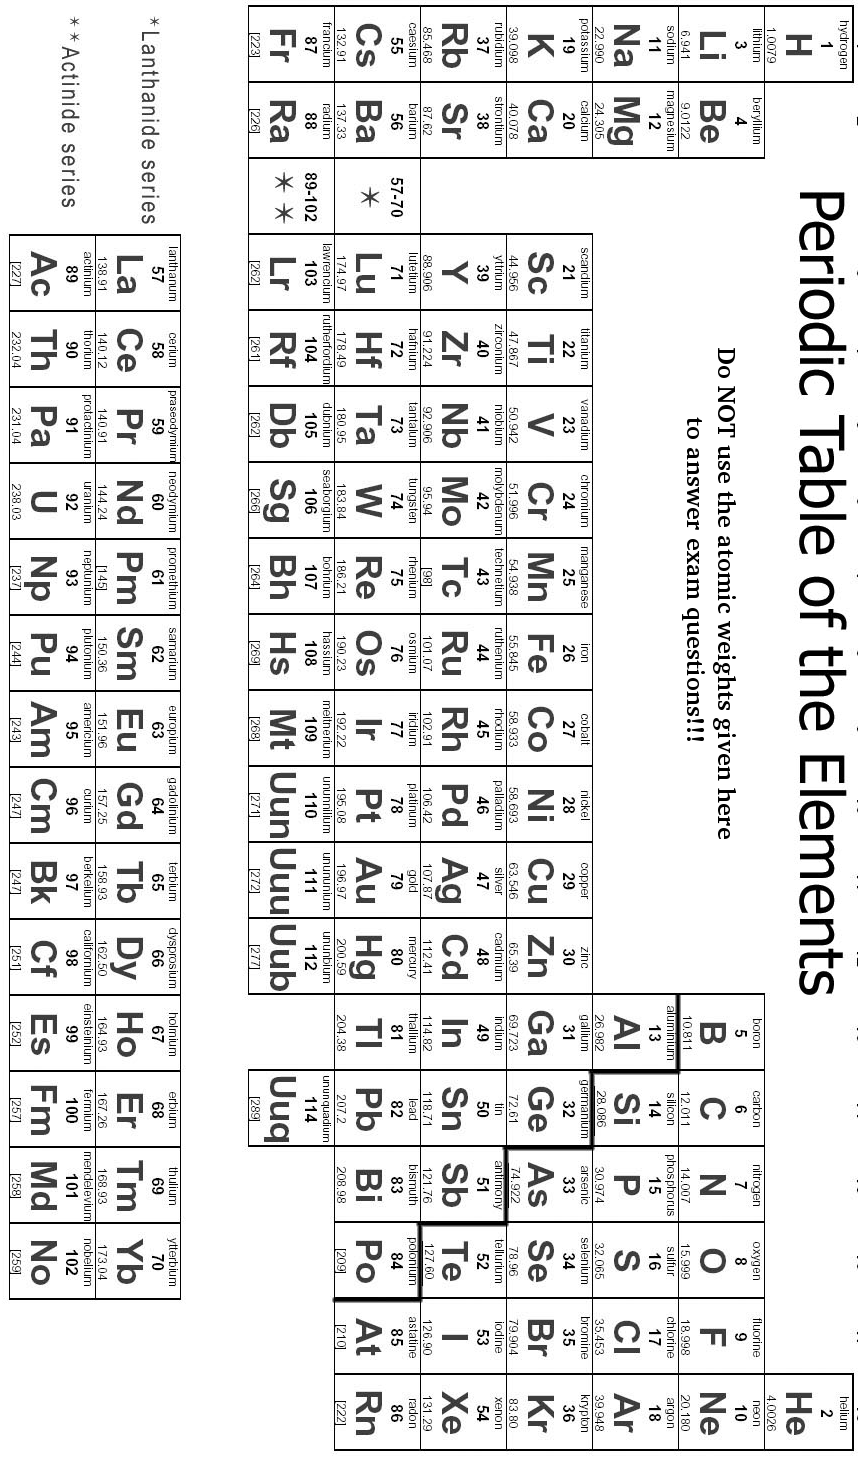
\includegraphics[width=4.5in]{pte.png}
\end{center}
\end{document}

\pagebreak





\problem{Chemical Driving Forces}{5}

Steam cracking is an important industrial process used to break down
hydrocarbons. Consider the cracking of butane (C$_4$H$_{10}$) into
ethene and ethane in the gas phase.

\begin{enumerate}

\item Formulate the balanced chemical equation for this process. Include
  states.

\item  determine the standard
  enthalpy of reaction and the standard free energy of reaction, both in
  kJ/mol.

  \begin{center}
    \begin{tabular}{lll}
      Compound & $\Delta$ H$_f^{\circ}$ (kJ/mol) & $\Delta$
      G$_f^{\circ}$ (kJ/mol) \\
      \hline
      Butane (g) & $-125.7$ & $-15.71$ \\
      Ethane (g) & $-84.68$ & $-32.0$  \\
      Ethene (g) & $52.4$ & $68.4$ 
    \end{tabular}
  \end{center}
    
  \item Estimate the temperature $T_c$ in K at which the reaction
    becomes spontaneous. What is the value of the equilibrium constant
    at $T_c$?
    
\end{enumerate}
